\documentclass{article}


\usepackage[english]{babel}
\usepackage{listings}

\usepackage[letterpaper,top=2cm,bottom=2cm,left=3cm,right=3cm,marginparwidth=1.75cm]{geometry}

% Useful packages
\usepackage{amsmath}
\usepackage{graphicx}
\usepackage[colorlinks=true, allcolors=blue]{hyperref}

\title{COSC/MATH 343 homework 1}
\author{Micah Sherry}

\begin{document}
\maketitle

\begin{enumerate}

\item Assume that you are solving the quadratic equation $ ax^2 + bx + c = 0 $, 
with $ a = 1.22 $, $ b = 3.34 $, 
and $ c = 2.28 $, using a normalized floating-point system with base = 10, $ p = 3 $ 
(the mantissa has only three digits). That is all numbers in the system are of the form:
$$ (0.d_1d_2d_3)_{10} \times 10^{\pm k}$$


where $d1 \neq 0$ 
    \begin{enumerate}
        \item What is the computed value of the discriminant $ b^2- 4ac$? 
        \\ The first step I took was to find $b^2$ in this floating point system for that I got $b^2 = .111 \times 10^2$. the next step I took was to calculate $ a \times c$ and for that I got $ a \times c = .270 \times 10^1$. then I multiplied that value by 4 to get $ 4\times a \times c = .108 \times 10^2 $. finally putting everything together I got $b^2 - 4\times a \times c = .300\times 10^{-2}$
        \item What is the exact value of the discriminant in real (exact) arithmetic?
        \\ the exact value for the discriminate $ \approx .0292 $
        \item What is the relative error in the computed value of the discriminant?
        \\ the relative error is calculated with $$ \frac{|true - approx|}{|true|}$$ using this formula I got $$\frac{|0.0292 - 0.003|}{|0.0292|}= 0.897$$
    \end{enumerate}

\item The harmonic series is known to diverge to $\infty$. The nth partial sum approaches ∞ at the same rate as ln(n). Euler’s constant is defined to be
$$\gamma = \lim_{n \to \infty } \left( \sum_{k=1}^{n}\frac{1}{k} - ln(n) \right)\approx 0.57721$$
\begin{enumerate}
    \item what is the largest value of s it would obtain? \\let $\epsilon_{mach} $ denote the machine precision   $$\epsilon_{mach} \approx 10^{-16}$$ 
    so the loop used to calculate the harmonic series will stop being accurate after $$ \frac{1}{k} < \epsilon_{mach}$$ where k is the number of iterations of the loop. 
    using algebra we find that the $$\frac{1}{\epsilon_{mach}} < k$$ meaning that using this loop the harmonic series will stop being accurate after the $10^{16}th$ iteration of the loop. to find the max value of the nth partial sum I will use the fact that $$0.57721+ln(n)\approx \sum_{k=1}^{n}\frac{1}{k}$$ Then substituting $10^{16}$ in for n we find the maximum value of s we can compute in this way is $$s \approx 37.42$$
    \item Write and test a program that uses a loop of at least 5000 steps to estimate Euler’s constant and Make a plot of the values
\begin{figure}[hbt!]
        \centering
        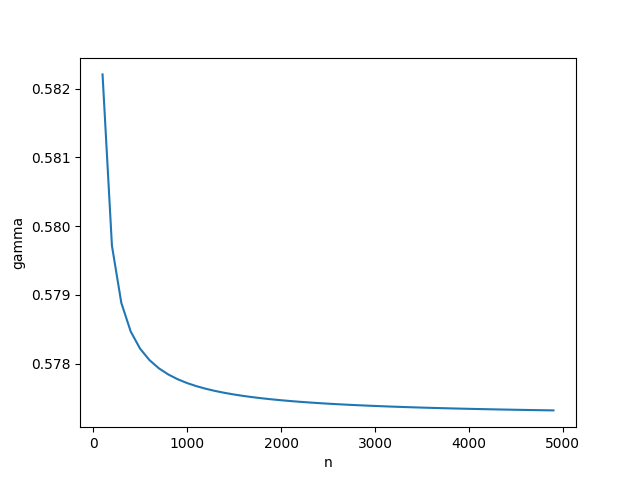
\includegraphics[width=1\linewidth]{gamma.png}
        \caption{$\gamma $ approximation}
        \label{fig:\gamma approximation}
    \end{figure}
    
\end{enumerate}
 
\pagebreak
\item Write a program to compute an approximate value for the derivative of a function
using the finite-difference formula
$$ f^{\prime}(x) \approx \frac{f(x+h)-f(x)}{h}$$
Test your program using the function tan(x) for x = 1. Determine the error by
comparing with the square of the built-in function sec(x). 
for the magnitude of the error.
    \begin{figure}[hbt!]
        \centering
        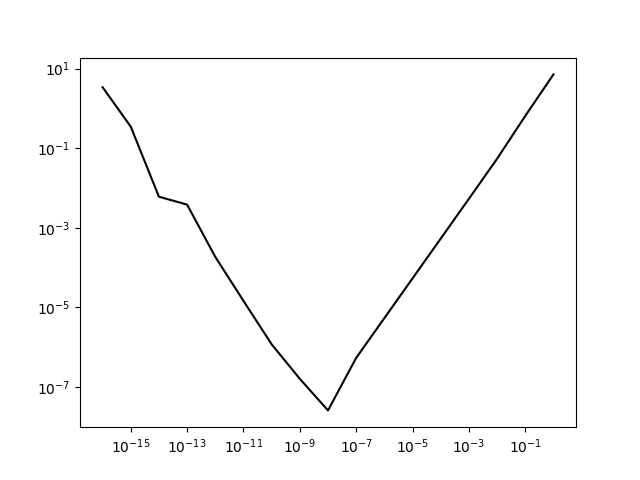
\includegraphics[width=1\linewidth]{finite_diff.png}
        \caption{ finite difference}
        \label{fig: finite diffrence}
    \end{figure}
    

    \begin{enumerate}
        \item Is there a minimum value for the magnitude of the error?
        \\ There is a local minimum at the $ h \approx 10^{-8} $
        \item How does the corresponding value for h compare with the value $ h \approx \sqrt{\epsilon_{mach}}$ where $\epsilon_{mach} \approx 10^{-16}$ is the machine precision value found in class examples? \\
        the value of h where there is a minimum is the square root of is $\epsilon_{mach}$
        \item Repeat the exercise using the centered difference approximation
        $$ f^{\prime}(x) \approx \frac{f(x+h)-f(x-h)}{2h}$$
        \\ using this formula the error reaches a minimum faster it reaches  a minimum at $ h \approx 10^{-7} $
        \begin{figure}[hbt!]
        \centering
        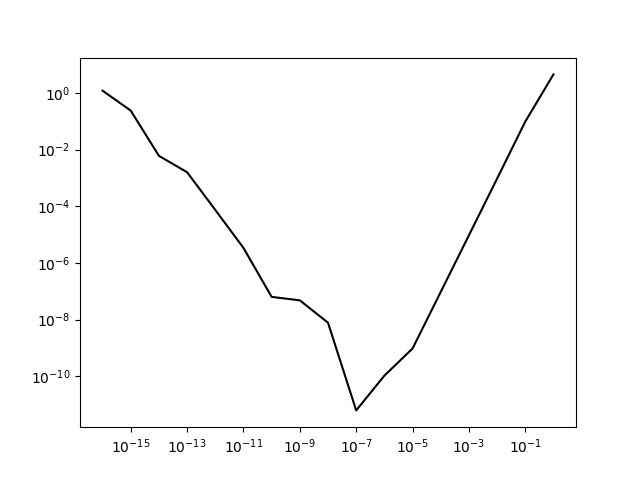
\includegraphics[width=1\linewidth]{finite_diff2png.png}
        \caption{ symmetric finite difference}
        \label{fig: symmetric finite diffrence}
        
    \end{figure}
    \end{enumerate}

\end{enumerate}

\end{document}